\documentclass[letterpaper, 12pt]{article}
\usepackage{aaai18}
\usepackage{times}
\usepackage{helvet}
\usepackage{courier}
\usepackage{url}
\usepackage{graphicx}
\usepackage{indentfirst}
\usepackage{adjustbox}
\usepackage{blindtext}
\frenchspacing

\graphicspath{ {images/} }

\title{Name A Bird: Fine-Grained Classification of Bird Images}
\author{Tao Jiashu \ Li Zeyong \  Wu Zhaoxuan \ Qian Peisheng \ He Yuchen \ Ding Xiangfei\\
National University of Singapore}
\date{}
\begin{document}
\maketitle

\begin{abstract}
Fine grained classification.
\end{abstract}

\section{Introduction}
The computer vision systems recently experienced substantial development in terms of
performance, through researches that exploits large scale visual datasets like the ImageNet.
ImageNet was formally a project aimed at labelling and categorising thousands of object classes,
but many pre-trained networks based on ImageNet have demonstrated excellent ability to generalise
to images outside the dataset via transfer learning. This suggests the possibility for many
interesting applications of image recognition classifiers learned through Machine Learning (ML).
Instead of recognising classes of day-to-day objects, this paper aims to build a more specific
classifier for different species of birds. The machine is much more likely to surpass human-level
performance of classifying specialised domains such as bird species, as compared to conventional
daily objects. Therefore, the use cases of this application are justified by the remarkable
accuracy achievable.

Education is the main market that the proposed machine learning model should venture into.
Xing Se is a similar flower recognition app that provides recognition as well as interesting
stories related to flowers that attracts numerous users in China. It reached the rank of top 6
in the China App Store under the category of Education. This paper aims to develop an accurate
model that can be applied to replicate the success in the context of Singapore.

\section{Individual contribution}

\section{Related work}
\subsection{Dateset}
The dataset used in this work is obtained from an openly available web resource named 
\textbf{Caltech-UCSD Birds (CUB)-200-2011} \cite{WahCUB_200_2011}.
The dataset consists of 11788 bird images of 200 species. Each image is annotated with 1
bounding box, 15 part locations and 312 binary attributes.

\subsection{AlexNet}
AlexNet \cite{Alex} is a famous convolutional neural network (CNN). It won the ImageNet Large Scale
Visual Recognition Challenge in 2012, achieving a top-5 error of 15.3\%, leading the first runners-up
by more than 10.8\%. It is acknowledged to be the model that popularised the use of CNNs in computer vision.

It was trained on more than 1 million images on ImageNet to output labels of the object in an image. AlexNet
is designed to classify objects into 1000 distinct subcategories.The original AlexNet consists of eight hidden layers where the first five
layers are convolutional and the remaining three are fully connected layers. The exact configurations
are listed below:
\begin{description}
	\item [conv1] 96 kernels of size $11 \times 11 \times 3$, stride = 4.
	\item [conv2] 256 kernels of size $5 \times 5 \times 48$, stride = 1.
	\item [conv3] 384 kernels of size $3 \times 3 \times 256$, stride = 1.
	\item [conv4, conv5] 384 kernels of size $3 \times 3 \times 192$, stride = 1.
	\item [FC6, FC7] 4096 fully connected neurons
    \item [FC8] 100 fully connected neurons (linear classifier)
\end{description}

\subsection{Fine-grained classification}
The 1000 subcategories of ImageNet images are very different in nature, for example, a cat and a car.
However, in the context of classifying bird species, the differences of birds are more subtle. Some
birds of different species may appear very similar, even difficult for humans to detect the differences.
This problem is fine-grained recognition, or classification, which is harder than normal categorisation problem.
Traditional methods use additional information such as part annotations of birds, to teach the computer how to
categorise birds. However, manual labelling of parts can be tedious. It is also very costly when scaling up to
large amount of data. Therefore, Krause et al. \cite{krause2015fine} proposed a method that does not use part annotations
to do fine-grained recognition.

They utilised bounding boxes of images to do foreground refinement, which greatly increases computer's ability
to detect the outlines of birds in a messy background.

\subsection{Cost-sensitive deep metric learning}
Zhao et al. \cite{Zhao} sharply points out the current deep learning loss function gives equal attention to all
subcategories. However, there usually exists some subcategories that are very similar to each other, and has very
high probability of being mis-classified. To address this issue, Zhao et al. \cite{Zhao} proposed a new loss function
that penalises more heavily on similar subcategories.

Confusion matrix is first calculated to find out the commonly mis-labelled subcategories.
\begin{figure}
    \begin{center}
        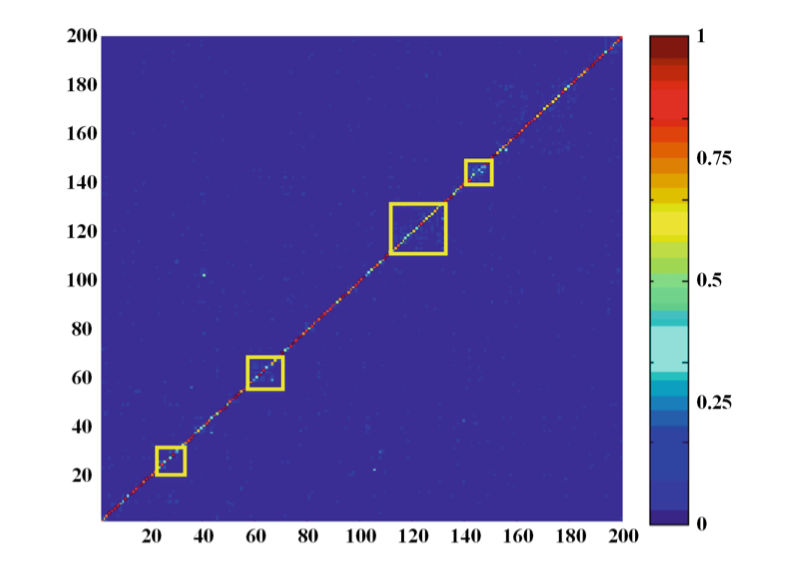
\includegraphics[width=0.5\textwidth]{confusion_matrix}
        \caption{Confusion matrix on CUB\_200\_2011 dataset. subcategories in yellow boxes are similar and easily mis-classified.\cite{Zhao}.}
    \end{center}
\end{figure}
As shown in Figure 1, Zhao et al. discovered that there are some subcategories that are often confused by the machine. They
subsequently incorporated the confusion matrix in the loss function and used weighted softmax to do linear classification.

\section{Our approach}
\subsection{Architecture}
There has been a few famous visual recognition models in the past twenty years.
From LeNet \cite{lecun1998gradient} in 1998, to AlexNet \cite{Alex} in 2012,
to GoogLeNet \cite{szegedy2015going}, also known as the Inception Network, in 2014,
to VGGNet \cite{simonyan2014very} in 2014 and ResNet \cite{he2016deep} in 2015, the
performance of image recognition models has drastically improved. However, as the performance
increases, the complexity of the deep learning network grows. To achieve a balance between
the performance and the complexity of the model, we decided to do a transfer learning
from AlexNet to implement this multiclass classification.

The original AlexNet is trained on ImageNet to classify images into 1000 categories.
In our project, there are only 200 categories of birds. Thus, we took away the last layer
of AlexNet and built a new linear classifier for 200 classes.

We kept all of the first seven layers of AlexNet because these early layers extracts general
features of images. Moreover, AlexNet was trained on 1 million images, while our dataset has only 5400
images in the training set. Our model, if train every single layer on our dataset, would not perform as
well as AlexNet in extracting the basic features. Training such a deep model with such small amount of
images also incurs great risks of overfitting. Therefore, due to these considerations, we adopted the
pre-trained weights of AlexNet and froze gradient descent in the first seven layers. In this way, our model
only does gradient descent on the parameters in the linear classifier layer. It greatly reduces the
training time and complexity of our model while retain the large part of feature extraction capabilities of
AlexNet.

\subsection{Optimisation}
We chose to do minibatch gradient descent to achieve a balance between training time for each step and
variance of the stochastic gradient updates. The batch size is then empirically chosen to be 128. We also
decided to use Adam optimiser because it works best with minibatch gradient descent.

\section{Performance and adjustment}
After 10 epochs, the validation accuracy rose from 20\% to 30\%. 10 more epochs did not bring significant
improvement to validation accuracy. Due to the stochastic nature of minibatch gradient descent, we run
the training process on several machines in order to achieve the best result. After 160 epochs of training,
the best model achieved 48\% on validation accuracy. The state-of-the-art model \cite{gavves2015local} that does not use
additional information such as the bounding boxes and part annotation achieves 53.6\% accuracy \cite{krause2015fine}
on the same dataset and with the same training-test set split. Thus, our best model is only 5.6\% down by
the state-of-the-art method.

We then tried He initialisation to randomly initialise the two parameters in the linear classifier in order to
achieve faster convergence. However, this time round, the accuracy gets stuck at 30\%. To analyse the training process,
we added TensorBoard integration to our model so that the training process can be visualised. After plotting a graph
of training accuracy and the cross-entropy loss, we found out that there may be a problem of overfitting.
\begin{figure}
    \begin{center}
        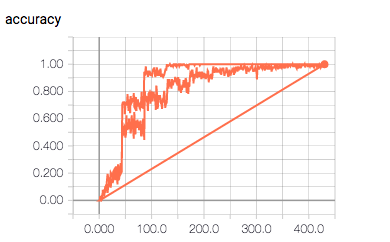
\includegraphics[width=0.5\textwidth]{training_accuracy}
        \caption{Training accuracy against steps in a vanilla model (up). Training accuracy against steps using dropout (mid).}
    \end{center}
\end{figure}

\begin{figure}
    \begin{center}
        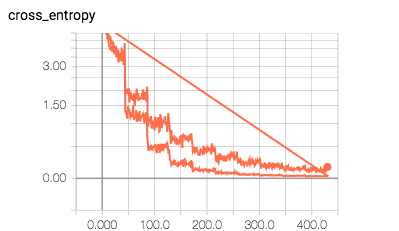
\includegraphics[width=0.5\textwidth]{cross_entropy}
        \caption{Cross-entropy loss against steps in a vanilla model (bottom). Cross-entropy loss against steps using dropout (mid).}
    \end{center}
\end{figure}

As shown in Figure 2 and 3, the training accuracy is almost 100\% at the 150th training step. The cross-entropy loss is also
very small after the 200th training step. In this case, the gradient is very small and the curve is almost flat. It is
a plateau and training becomes very slow. Moreover, the validation accuracy is only at 30\%. The huge gap between training
accuracy and validation accuracy suggests that our model does not generalise well and encounters overfitting.

\subsection{Dropout}
To tackle overfitting, there are three common ways:
\begin{center}
    \begin{enumerate}
        \item Input more data
        \item Reduce model complexity
        \item Dropout
    \end{enumerate}
\end{center}

We chose to do dropout with a dropout probability of 0.5 as it does best in tackling overfitting.
After adding the dropout process between FC7 and FC8, the model structure is shown in Figure 4.
\begin{figure*}
    \begin{center}
        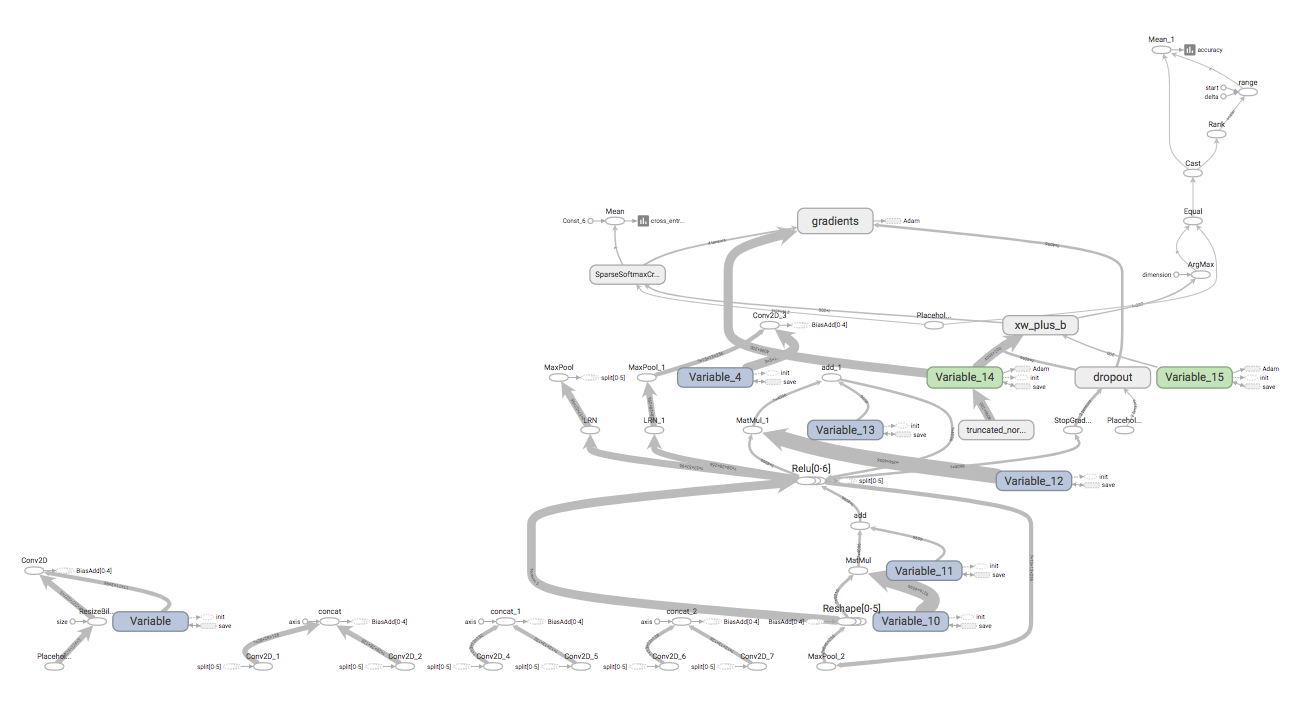
\includegraphics[width=\textwidth]{structure}
        \caption{Structure of our model after adding dropout.}
    \end{center}
\end{figure*}
After training the new model with dropout for 400 steps, the validation accuracy is at 29\% while the training accuracy again
gets very close to 1. Although the cross-entropy loss is larger, the gradient is flat and the training process gets stuck.
After training for more epochs, we found out that dropout with a \texttt{keep\_prob = 0.5} is not enough to solve the problem of
overfitting. The validation accuracy is lower, and the time of convergence is doubled.

The reason behind the severe overfitting is probably the outstanding capabilities of AlexNet in extract features from images. It was
designed to train on 1 million images. Since we have have 0.5\% of the amount of images it was trained on in the training set, AlexNet
is able to overfit them in the training process. Moreover, the similarity between subcategories in fine-grained recognition makes
mis-classification much easier when the input data is insufficient. Therefore, dropout is not enough in addressing overfitting.

\subsection{Cost sensitive deep metric learning}
We then attempted to address the problem by using the alternative cost function introduced by Zhao et al. \cite{Zhao}.
We first computed the confusion matrix $C$ from the label and predictions by using the built-in function in TensorFlow. Then we modified
the softmax function as the following:
$$weighted\_softmax(I,L)=\frac{1}{n}\sum^n_{i=1}-W_i\times log(s_i^{L_i})$$
where $I$ is the image space, $L$ is the category space, and
$$W_i=\sum^k_{j=1,j\not =i}C_{ij}$$
$$s_i^{L_i}=\frac{\frac{1}{k}\times e_f(I_i,L_i)}{\sum^k_{j=1}M_{ij}\times e_f(I_i,L_i)}$$

We did not use the built-in TensorFlow function \texttt{tf.nn.weighted\_cross\_entropy\_with\_logits} because according to its documentation, it
is a binary classification while we are doing a multiclass classification.

Therefore, we used \texttt{tf.nn.sparse\_softmax\_\\cross\_entropy\_with\_logits} to compute the original cross-entropy loss, and element wise multiply the
weight of each individual subcategories. However, we then realised that this new loss function has the similar gradient with respect to \texttt{FC8W} and
\texttt{FC8b}, which are the weight and bias terms in the linear classifier. The reason is that the partial derivative of the additional coefficients with
respect to the two parameters are 0, making them coefficients of the new gradient function. Hence, we simply multiply them to the gradients. However, this
caused an unexpected error. The gradient is of dimension equal to the batch size, while the coefficients are of dimension equal to the number of subcategories.
It is not feasible to implement this when the two dimensions do not match. We then manually re-wrote the cost function as Zhao et al. \cite{Zhao} proposed,
and the Adam optimiser encounters the same problem of dimension mismatch.

Unfortunately, Zhao et al. \cite{Zhao} did not publish their source code. We could not figure out how they implemented the weighted softmax and addressed the
issue of dimension mismatch. Therefore, after a few days of trying, we aborted this enhancement.

\subsection{Image augmentation}
After dropout failed to tackle the problem of overfitting, we resorted to increasing the size of input. However, it is costly to maunally download more pictures
of birds and label them one by one. Thus, we decided to do image augmentation. Common image augmentation techniques include translation, rotation, flipping, scaling
and PCA colour augmentation. We decided to add 10 more augmented images for each image in the training set, so that we would have around 54,000 images in the
training set. The image processing programme is taken from the source code of inception-v4 from Google.

Due to the limited computing power, we decided to use Google Colab to accelerate training with cloud GPUs. We ran the script over the night, and sadly discovered
that the runtime was terminated by Google. It is probably because it takes too much time to load our dataset and even more time to do image augmentation. Unfortunately,
we did not finish image augmentation and tested its performance.

\section{Application}
After training the model, we decided to make an application out of the neural network. The programme takes in the saved weight of all parameters in the model, and
takes in images uploaded by the user. We name our programme "Name A Bird" because we aim to inform users of the name of the bird from a bird image. Similar to AlexNet,
we decided to output the five most likely categories with their respective confidence level. The reason behind this is that our model is only 48\% accurate in
categorising birds. Only outputting the most likely category have a larger chance of making a mistake.

We did a few tests on the programme and the programme takes less than 1 second to output the five most likely categories of a bird for each single image input.

\bibliography{reference}
\bibliographystyle{unsrt}
\end{document}
